\chapter{How to integrate Dresden OCL2 for Eclipse}
\label{chapter:integration}

\begin{flushright}
\textit{Chapter written by Claas Wilke}
\end{flushright}

In Chapter \ref{chapter:architecture} the architecture of \acl{DOT4Eclipse} has shortly been explained. This chapter will explain, how \acl{DOT4Eclipse} can be integrated into other tools, toolkits or projects.



\section{The Integration Facade of Dresden OCL2 for Eclipse}

Since the release 2.1.0, \acl{DOT4Eclipse} contains an \keyword{Integration Facade}, that combines all required interfaces of \acl{DOT4Eclipse} in one interface, also called a \keyword{Facade} \cite{gamma:dp}. The facade contains self-explanatory static methods that provide access to the repository (modelbus) and all tools of \acl{DOT4Eclipse}. A documentation of the complete facade's interface would be too large for this documentation. Thus, please investigate the facade directly in the code. The facade called \code{Ocl2ForEclipseFacade} is located in the plug-in \code{tudresden.ocl20.pivot.facade}. Please be aware of the fact that if you use the facade, you will result in dependencies to all major parts of \acl{DOT4Eclipse}. Thus, if you want to use one of the tools only (e.g, the \acs{OCL}2 Parser) you could access these tools directly as explained below.



\section{How to access Meta-Models, Models and Instances}

The central component of \acl{DOT4Eclipse} is the \keyword{Model-Bus} which is implemented by the Eclipse plug-in \code{tudresden.ocl20.pivot.modelbus}. The main class of this plug-in (\code{tudresden.\linebreak[0]ocl20.pivot.modelbus.ModelBusPlugin}) provides methos, to access meta-models, models and model instances and to import new resources of these kinds into the toolkit (see Figure \ref{pic:integration:modelBusPlugin}).

The class provides four different static methods to access different registries, the \code{Meta\-model\-Re\-gis\-try}, the \code{ModelRegistry}, the \code{ModelInstanceTypeRegistry} and the \code{ModelInstanceRegistry}.

\begin{figure}[!b]
	\centering
	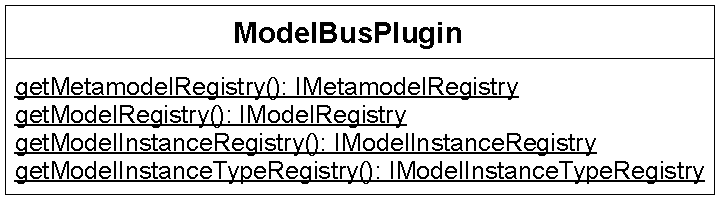
\includegraphics[width=.8\linewidth]{figures/integration/modelBusPlugin}
	\caption{The main class of the Model-Bus plug-in.}
	\label{pic:integration:modelBusPlugin}
\end{figure}


\subsection{The Meta-Model Registry}

The Meta-Model Registry provides methods to add and get meta-models to and from \acl{DOT4Eclipse}. Normally, the method \code{addMetamodel(IMetamodel)} is not required because by starting Eclipse, all meta-models register themselves via their extension point in the registry. To get a meta-model from the toolkit, the methods \code{getMetamodels()} and \code{getMetamodel(id: String)} can be used. The method \code{getMetamodels()} returns all meta-models that are currently registered in the registry. The method \code{getMetamodel(id: String)} can be used to get a meta-model by its ID (Normally, the ID of a meta-model is equal to the name of its plug-in. E.g., the \acs{UML}2 meta-model has the ID \code{tudresden.ocl20.pivot.metamodels.uml2}).

\begin{figure}[!b]
	\centering
	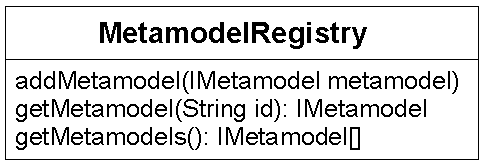
\includegraphics[width=.55\linewidth]{figures/integration/metaModelRegistry}
	\caption{The Meta-Model Registry.}
	\label{pic:integration:metaModelRegistry}
\end{figure}


\subsection{How to load a Model}

First, to load a model into \acl{DOT4Eclipse}, the meta-model the model is an instance of has to be selected . E.g., for an \acs{UML}2 class diagram the \acs{UML}2 meta-model should be selected (see Listing \ref{lst:integration:loadModel}). Each meta-model has its own \code{IModelProvider} that can be accessed by using the method \code{IMetamodel.getModelProvider()}. The \code{IModelProvider} provides three methods to load a model. A model can be loaded by using the method \code{getModel(..)} with

\begin{enumerate}
	\item A \code{File} object representing the model as argument,
	\item a \code{String} representing the path of the file there the model is located,
	\item or a \code{URL} leading to the file there the model is located.
\end{enumerate}

\lstset{
  language=Java
}
\begin{lstlisting}[caption={How to load a model.}, captionpos=b, label=lst:integration:loadModel, float]
IMetamodel metaModel;
IModel model;

metaModel = ModelBusPlugin.getMetamodelRegistry()
              .getMetamodel("tudresden.ocl20.pivot.metamodels.uml2");
model = metaModel.getModelProvider().getModel(modelURL);
\end{lstlisting}

\begin{figure}[!b]
	\centering
	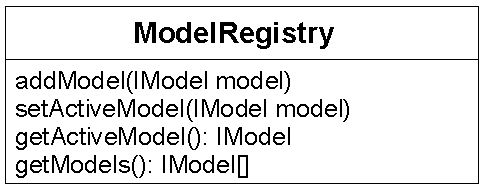
\includegraphics[width=.55\linewidth]{figures/integration/modelRegistry}
	\caption{The Model Registry.}
	\label{pic:integration:modelRegistry}
\end{figure}

After loading the model, the model can be added to the \code{ModelRegistry}, that manages all models currently loaded into \acl{DOT4Eclipse} (see Figure \ref{pic:integration:modelRegistry}). The \code{ModelRegistry} can also be used to set an active model which represents the \code{IModel} that is currently selected in the \keyword{Model Browser} of \acl{DOT4Eclipse}.


\subsection{The Model Instance Type Registry}

Similar to the Meta-Model Registry, the Model Instance Type Registry provides methods to add and get model instance types to and from \acl{DOT4Eclipse}. Normally, the method \code{addModelInstanceType(IModelInstanceType)} is not required because by starting Eclipse, all model instance types register themselves via their extension point in the registry. To get a model instance type from the toolkit, the methods \code{getModelInstanceTypes()} and \code{getModelInstance\-Type\linebreak[0](id: String)} can be used. The method \code{getModelInstanceTypes()} returns all model instance types that are currently registered in the registry. The method \code{getModelInstanceType(id: String)} can be used to get a model instance types by its ID (Normally, the ID of a model instance type is equal to the name of its plug-in. E.g., the Java model instance type has the ID \code{tudresden.ocl20.pivot.modelinstancetype.java}).

\begin{figure}[!b]
	\centering
	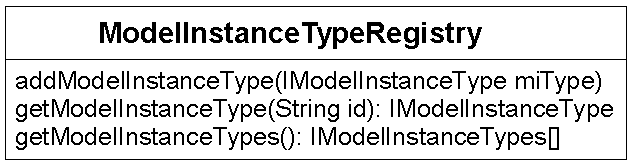
\includegraphics[width=.7\linewidth]{figures/integration/modelInstanceTypeRegistry}
	\caption{The Model Instance Type Registry.}
	\label{pic:integration:modelInstanceTypeRegistry}
\end{figure}


\subsection{How to load a Model Instance}

First, to load a model instance into \acl{DOT4Eclipse}, the model instance type must be selected the instance is an instance of. E.g., for a set of Java objects the Java model instance type should be selected (see Listing \ref{lst:integration:loadModelInstance}). Each model instance type has its own \code{IModelInstanceProvider} that can be accessed by using the method \code{IModelInstanceType.get\-Mo\-del\-Instance\-Provider}. The \code{IModelInstanceProvider} provides three methods to load a model instance. A model instance can be loaded by using the method \code{getModelInstance(..)} with

\begin{enumerate}
	\item A \code{File} object representing the model instance as argument,
	\item a \code{String} representing the path of the file there the model instance is located,
	\item or a \code{URL} leading to the file there the model instance is located.
\end{enumerate}

Additionally, each of these methods requires the \code{IModel} as a second argument, the model instance is an instance of. Thus, the model must be loaded before the model instance can be loaded.

\lstset{
  language=Java
}
\begin{lstlisting}[caption={How to load a model instance.}, captionpos=b, label=lst:integration:loadModelInstance, float]
IModelInstanceType miType;
IModelInstance modelInstance;

miType = ModelBusPlugin.getModelInstanceTypeRegistry()
           .getModelInstanceType(
             "tudresden.ocl20.pivot.modelinstancetype.java");
modelInstance = miType.getModelInstanceProvider()
                  .getModelInstance(modelInstanceUrl, model);
\end{lstlisting}

\begin{figure}[!b]
	\centering
	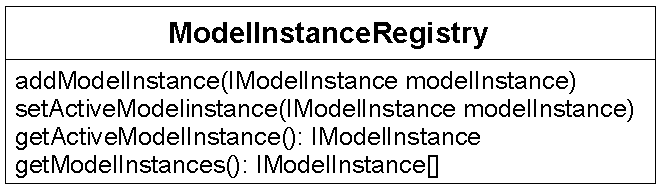
\includegraphics[width=.75\linewidth]{figures/integration/modelInstanceRegistry}
	\caption{The Model Instance Registry.}
	\label{pic:integration:modelInstanceRegistry}
\end{figure}

After loading the model instance, the model instance can be added to the \code{Model\-Instance\-Re\-gis\-try}, that manages all model instances currently loaded into \acl{DOT4Eclipse} (see Figure \ref{pic:integration:modelInstanceRegistry}). The \code{ModelInstanceRegistry} can also be used to set an active model instance that represents the \code{IModelInstance} that is currently selected in the \keyword{Model Instance Browser} of \acl{DOT4Eclipse}.



\section{How to access the OCL2 Parser}

The \acs{OCL}2 Parser of \acl{DOT4Eclipse} is located in the plug-in \code{tudresden.ocl20.pivot.\linebreak[0]ocl\-2\-Parser}. The parser provides a very simple interface and can be used as shown in Listing \ref{lst:integration:parserConstraints}. First a \code{Reader} used to read all constraints that shall be parsed has to be created, and an \code{IModel} for that the constraints shall be parsed has to be loaded. Afterwards, the method \code{OCL2Parser.doParse()} can be invoke on the singleton instance of the parser to parse the constraints.

\begin{figure}[!b]
\begin{lstlisting}[caption={How to parse constraints.}, captionpos=b, label=lst:integration:parserConstraints]
FileReader oclFileReader;
OCL2Parser parser;
List<Constraint> parsedConstraints;

oclFileReader = new FileReader(oclFile);
parsedConstraints = Ocl2Parser.INSTANCE.doParse(model, reader);
\end{lstlisting}
\end{figure}



\section{How to access the OCL2 Interpreter}

To use the \acs{OCL}2 Interpreter, a model and a model instance must be loaded into the toolkit before. Additionally, at least one constraint must be parsed that shall be interpreted for the objects contained in the model instance. The interpreter is located in the plug-in \code{tudresden.ocl20.pi\-vot.\linebreak[0]in\-ter\-pre\-ter}. It has a more complex interface than the other tools and contains many different operations to interpret different kinds of constraints.

\begin{figure}[!b]
\begin{lstlisting}[caption={How to interpret constraints.}, captionpos=b, label=lst:integration:interpretConstraints]
IModel model;
IModelInstance modelInstance;

/*
 * Load model, model instance and constraints. ...
 */

IOclInterpreter oclInterpreter;

List<Constraint> constraints;
List<IModelInstanceObject> modelInstanceObjects;
List<IInterpretationResult> results;

oclInterpreter = OclInterpreterPlugin.createInterpreter(modelInstance);

constraints = model.getRootNamespace().getOwnedAndNestedRules();
modelInstanceObjects = modelInstance.getAllModelInstanceObjects();

results = new ArrayList<IInterpretationResult>();

for (IModelInstanceObject aModelInstanceObject : modelInstanceObjects) {
  results.addAll(oclInterpreter.interpretConstraints(constraints,
  	aModelInstanceObject));
}
\end{lstlisting}
\end{figure}

Listing \ref{lst:integration:interpretConstraints} shows how the \code{OclIntepreter} can be used. First, a model and a model instance must be loaded on which the constraints shall be verified. Furthermore, at least one constraint must be parsed that shall be interpreted (lines 1-6). Afterwards, an \code{IOclInterpreter} can be created for the loaded model instance by using the factory method of the \code{OclInterpreterPlugin} (line 14). Finnaly, the parsed constraints can be interpreted for all \code{IModelInstanceObjects} of the model instance by iterating over them (lines 21-24). The result of each interpretation will be an \code{IInterpretationResult} which internally contains a triple of (1) an \code{IModelInstanceObject} on which (2) a \code{Constraint} have been interpreted resulting in (3) an \code{OclAny}.



\section{Summary}

This chapter shortly presented, how the tools of \acl{DOT4Eclipse} can be accessed and used via their interfaces. First, the integration facade has been presented, afterwards, direct access of specific tools and the modelbus has been explained. Please be aware of the fact, that direct code documentation is always error-prone and will be outdated very soon. Thus, please do not hesitate to contact us if some parts of this chapter are written in a unclear manner or are inconsistent with the code.